
\chapter{Izvedba}

Sustav kreiran kao prakti\v{c}ni dio ovog rada sastoji se od mobilne i internetske aplikacije te je shodno tome ovo poglavlje podijeljeno u dva dijela u kojima su opisane korit\v{s}tene tehnologije i alati te motivi za njihov odabir. Iako su aplikacije iz razli\v{c}itih podru\v{c}ja ra\v{c}unarstva, razvoj im je organiziran i vo\dj en na isti na\v{c}in, koriste\'{c}i alat Git \cite{git}. Git je alat koji je kreirao tim Linusa Torvaldsa, oca Linuxa i jednog od najbitnijih i zna\v{c}ajnijih in\v{z}enjera u ra\v{c}unarstvu, za potrebe razvoja jezgre Linux-a. Git slu\v{z}i za verzioniranje i organizaciju koda i funkcionira na na\v{c}in da korisnik grupira napravljene promjene u cjeline (commit-ove) koji \v{c}ine logi\v{c}ke cjeline (branch-eve) koje obi\v{c}no predstavljaju funkcionalnosti aplikacije. Na taj na\v{c}in je cijeli razvoj projekta evidentiran i u bilo kojem trenutku se mo\v{z}e vratiti na bilo koje pro\v{s}lo stanje. Posebno je koristan u organizaciji ve\'{c}ih timova jer omogu\'{c}ava da vi\v{s}e ljudi radi na razli\v{c}itim dijelovima projekta, \v{c}ak i na istom kodu jer posjeduje mehanizam za rje\v{s}avanje konflikata nastalih ure\dj enjem iste linije koda od vi\v{s}e razli\v{c}itih programera. 

U praksi se koriste i razli\v{c}ite metode kori\v{s}tenja Git-a, od kojih je naj\v{c}e\v{s}\'{c}e kori\v{s}tena ``Git flow'' \cite{git_flow}, koja specificira organizaciju branch-eva s ciljem standardizacije i efektivnijeg kori\v{s}tenja Git-a. Nadalje, u praksi se Git koristi u kombinaciji sa platformama za pohranjivanje projekata \v{s}to omogu\'{c}uje decentralizaciju projekta, suradnju vi\v{s}e programera i sigurnost (rezervna kopija je na serveru). Oba projekta koriste platformu Github \cite{github} koja je jedna od najkori\v{s}tenijih platformi za projekte otvorenog koda. Uz navedene prednosti, Github pru\v{z}a i dodatne statistike i informacije o projektu, kao npr. graf napravljenih commitova u vremenu, prikazan na slici  ~\ref{fig:commits}.

\begin{figure}[!htbp]
	\begin{center}
 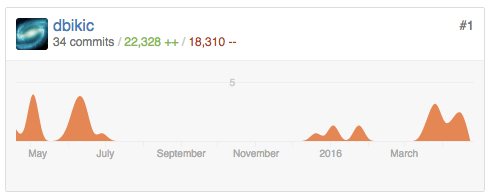
\includegraphics[height=4.2cm,keepaspectratio=true]{git_commits}
 \caption{Graf commit-ova u vremenskom periodu za projekt mobilne aplikacije}
 \label{fig:commits}
	\end{center}
\end{figure}

\section{Mobilna aplikacija}

\subsection{Tehnologija}
Klijentska mobilna aplikacija je razvijena za Android operativni sustav, \v{c}iji je logo prikazan na slici ~\ref{fig:android}. Android je baziran na Linux jezgri te je kao takav projekt otvorenog koda. Razvoj Androida vodi tvrtka Google (2005. godine Google kupuje tvrtku Android Inc. koja je po\v{c}ela sa razvojem Android-a \cite{kupnjaAndroida}) koja u suradnji s proizvo\dj a\v{c}ima pametnih telefona kreira Android operativni sustav koji je instaliran na ve\'{c}ini ure\dj aja na tr\v{z}i\v{s}tu.
Takav Android nije u potpunosti otvorenog koda jer uklju\v{c}uje aplikacije koje nisu otvorenog koda (najva\v{z}nija je Google Play \cite{googlePlay}, centralna platforma za distribuciju aplikacija, glazbe i filmova).

\begin{figure}[!htbp]
	\begin{center}
 
\includegraphics[height=4cm,keepaspectratio=true]{android}
 \caption{Logo Android-a}
 \label{fig:android}
	\end{center}
\end{figure}

Zbog otvorenosti koda i mogu\'{c}nosti da svaki proizvo\dj a\v{c} kreira svoju verziju sustava (sa Google-ovim modulima ili bez), Android je danas najrasprostranjenija mobilna plaforma - danas svako drugo kupljeno ra\v{c}unalo ima instaliran Android operativni sustav \cite{androidDominacija}.

Aplikacije za Android platformu se razvijaju u Java programskom jeziku, na na\v{c}in da se jezgra Java-e pro\v{s}iri sa Android SDK-om (skup alata, biblioteka i dokumentacije koji skupa \v{c}ine platformu za razvoj Android aplikacija). Danas postoji vi\v{s}e alternativa Javi, prvenstveno zbog zastarjelosti Jave koja je razvijena po\v{c}etkom 1990. godine. Jedna od najkvalitetnijih novih alternativa je programski jezik Kotlin \cite{kotlin}. 

Android aplikacije se na pametnom telefonu izvr\v{s}avaju na na\v{c}in da se za svaku aplikaciju u okolini za izvr\v{s}avanje kreira instanca virtualnog stroja. 
Virtualni stroj pokre\'{c}e aplikacije pokre\'{c}u\'{c}i .dex datoteke koje se dobivaju prevo\dj enjem bytecode datoteka aplikacije, koje nastaju prevo\dj enjem izvornih .java datoteka i tako stvaraju okru\v{z}enje za razvoj Android aplikacija. Do Android verzije 5.0 se za okru\v{z}enje za izvr\v{s}avanje koristilo Dalvik VM okru\v{z}enje, koje je kod svakog pokretanja aplikacije prevodio bytecode u .dex datoteke. Od Android 5.0 se koristi ART okru\v{z}enje koje vr\v{s}i prevo\dj enje bytecode datoteka unaprijed, odnosno prilikom instalacije aplikacije. Na taj na\v{c}in se smanjuje broj prevo\dj enja \v{s}to rezultira smanjenjem kori\v{s}tenja procesora ure\dj aja i smanjenjem potro\v{s}nje baterije \cite{dalvikArt}.



\subsection{Alati}
Razvoj Android aplikacija se vr\v{s}i u integriranom razvojnom okru\v{z}enju Android Studio \cite{androidStudio}. Baziran je na okru\v{z}enju IntelliJ IDEA \cite{inteliJ} tvrtke JetBrains (ista tvrtka koja razvija programski jezik Kotlin \cite{kotlin}). Programerima pru\v{z}a razne funkcionalnosti koje uklju\v{c}uju:

\begin{itemize}
		\item Sustav izgradnje baziran na sustavu Gradle \cite{gradle}
		\begin{itemize}
			\item Pru\v{z}a jednostavno verzioniranje aplikacija, dodavanje knji\v{z}ica, testiranje aplikacije
		\end{itemize}
		\item Omogu\'{c}avanja izgradnje razli\v{c}itih verzija iste aplikacije
		\begin{itemize}
			\item Korisno ako programer \v{z}eli napraviti besplatnu i pla\'{c}enu verziju aplikacije ili imati verziju aplikacije za testno i produkcijsko okru\v{z}enje
		\end{itemize}
		\item Intuitivni ure\dj iva\v{c} korisni\v{c}kih su\v{c}elja
	\end{itemize}


\section{Internetska aplikacija}

\subsection{Tehnologije}

Internetska aplikacija sastoji se od dva dijela: klijentskog i poslu\v{z}iteljskog. Iako se oba dijela nalaze na istom poslu\v{z}itelju, razlika izme\dj u njih je u lokaciji na kojoj se kod izvr\v{s}ava. Klijentski dio se izvr\v{s}ava u korisni\v{c}kom pregledniku te uklju\v{c}uje korisni\v{c}ko su\v{c}elje aplikacije, dok se poslu\v{z}iteljski dio izvr\v{s}ava na poslu\v{z}itelju i uklju\v{c}uje bazu podataka te su\v{c}elje za pristupanje bazi.

Korisni\v{c}ko su\v{c}elje kreirano je uz pomo\'{c} tri standardne internetske tehnologije koje su temelj interneta kakav je danas: HTML, CSS i Javascript. HTML \cite{html} je standardni jezik za kreaciju elemenata internetske stranice i temelj za sav daljnji dizajn i logiku. CSS \cite{css} slu\v{z}i za definiranje stilova koji se dodaju HTML elementima i koje preglednik interpretira te na temelju njih definira izgled, poziciju i pona\v{s}anje elemenata. Javascript \cite{javascript} se koristi za interakciju korisnika i internetske stranice, te za manipulaciju HTML elemenata.

Poslu\v{z}iteljska strana uklju\v{c}uje MySQL \cite{mysql} bazu podataka i PHP \cite{php} skripte koje dohva\'{c}aju podatke iz nje te ih u obliku HTML elemenata prikazuju na korisni\v{c}kom su\v{c}elju. MySQL je sustav za upravljanje bazama podataka koji uklju\v{c}uje relacijsku bazu podataka kojom se upravlja pomo\'{c}u SQL jezika. PHP je skriptni jezik koji se koristi na poslu\v{z}iteljskoj strani za komunikaciju s bazom. Funkcionira tako da se u HTML kod ugra\dj uje skriptni kod kojeg poslu\v{z}itelj prepoznaje i izvr\v{s}ava, te se rezultat izvr\v{s}avanja ispisuje u HTML kod koji se \v{s}alje klijentu.

Opisane tehnologije su izabrane prvenstveno jer su sve otvorenog koda, a zatim jer su standard u domeni internetskih aplikacija (HTML, CSS, Javascript) i \v{c}esto se koriste u praksi (MySQL, PHP).

\subsection{Alati}
Kori\v{s}teni alati za izradu internetske aplikacije su:
\begin{itemize}
	\item Atom 1.6.2 \cite{atom}
	\begin{itemize}
		\item Ure\dj iva\v{c} koda koji je razvila tvrtka GitHub
		\item Kori\v{s}ten za pisanje svog koda (HTML, CSS, Javascript i PHP)
	\end{itemize}
	
	\item XAMPP 5.6.12-0 \cite{xampp}
	\begin{itemize}
		\item Paket alata namjenjen za poslu\v{z}itelje koji uklju\v{c}uje HTTP poslu\v{z}itelj, MySQL bazu podataka i interpreter programskih jezika PHP i Pearl
		\item Kori\v{s}ten je za kreiranje lokalnog testnog poslu\v{z}itelja i za kreiranje i administraciju baze podataka pomo\'{c}u alata phpMyAdmin
	\end{itemize}
	
	\item FileZilla 3.16.1 \cite{filezilla}
	\begin{itemize}
		\item Klijent za SFTP prijenos datoteka na poslu\v{z}itelj
	\end{itemize}
\end{itemize}